\documentclass[aspectratio=169,14pt,usenames,dvipsnames]{beamer}

\usepackage[utf8]{inputenc}
\usepackage{enumitem}
\usepackage{calc}

\usepackage{datetime}
\newcommand\builddate{%
   \ifcase \month%
        \or Janeiro%
        \or Fevereiro%
        \or Março%
        \or Abril%
        \or Maio%
        \or Junho%
        \or Julho%
        \or Agosto%
        \or Setembro%
        \or Outubro%
        \or Novembro%
        \or Dezembro%
    \fi\space\number\year%
}

\newcommand{\loadtheme}[1]{%
    \input{themes/#1}%
}
\newcommand{\presentationlanguage}[1]{%
    \usepackage[#1]{babel}%
}

\newcommand{\usecodingsamples}[1]{%
    \usepackage{listings}%
    \input{listings/#1}%
}

% Configura a apresentação para ser executada em tela cheia.
\newcommand{\setfullscreen}{\hypersetup{pdfpagemode=FullScreen}}

% Hide beamer navigation simbols
\beamertemplatenavigationsymbolsempty

%
% Standard frames
%

% coverframe
\newcommand{\coverframe}{%
    \begin{frame} %
        \titlepage %
    \end{frame} %
}

% finalframe{email}
\newcommand{\finalframe}[2][Thank you!]{%
    \begin{frame}%
        \begin{flushright}%
            \huge \textbf{#1}%
            \vfill%
            \large \textbf{#2}%
        \end{flushright}%
    \end{frame}%
}

\newcommand{\bigtitle}[1]{%
    \begin{frame}%
        \begin{center}%
            \Huge {#1}%
        \end{center}%
    \end{frame}%
}



\loadtheme{tchelinux}
\usecodingsamples{python}

\title[]{O TCC... um dia ele chega!}
\subtitle[]{\emph{The beautiful and easy \LaTeX\ way.}}
\author[]{Rafael Guterres Jeffman}
% dirty hack, since date is much larger than 'institute'
\institute[]{}
\date{Tchelinux}


% Configura a apresentação para ser executada em tela cheia.
\hypersetup{pdfpagemode=FullScreen}

% Hide beamer navigation simbols
\beamertemplatenavigationsymbolsempty

% Centraliza os títulos dos slides.
\setbeamertemplate{frametitle}[default][center]

% Ajusta a imagem de fundo padrão para a arpesentação.
\usebackgroundtemplate{
    \includegraphics[width=2cm]{\tuxgaucho}
}

\begin{document}

\begin{frame}
    \titlepage
\end{frame}

\begin{frame}[c]
    \frametitle{O Drama do TCC}
    \begin{itemize}
    \item{O que eu faço?}
    \item{Por que eu faço?}
    \item{Como eu faço?}
    \item{Com o que eu faço?}
    \item{Onde eu faço?}
    \end{itemize}
\end{frame}

\begin{frame}
    \vfill
    \begin{center}
    \large Essa é parte fácil, porque depois de tudo ainda tem as...
    \end{center}
\end{frame}

\begin{frame}[t]
    \begin{tikzpicture}[remember picture,overlay]  
        % Posiciona o overlay na página
        \node [xshift=\paperwidth / 2, yshift=\paperheight / 2] at (current page.south west)
        % Adiciona a imagem, definindo seu tamanho
        {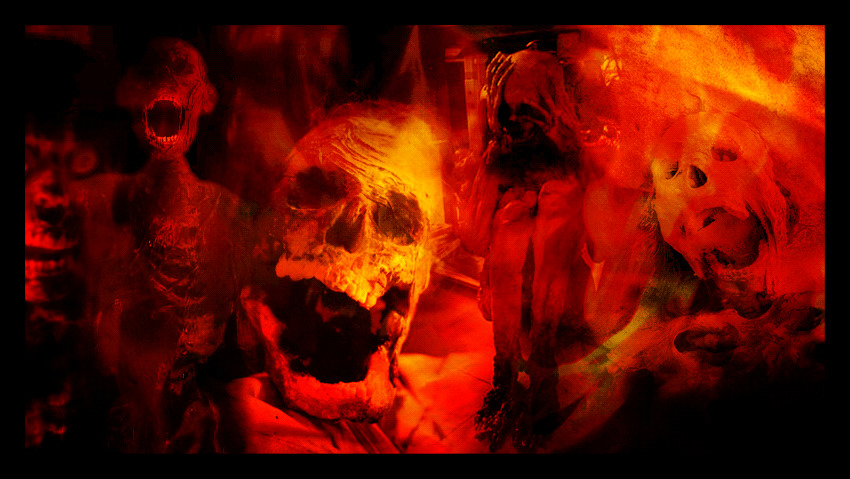
\includegraphics[height=\paperheight]{../../images/hell.jpg}};
    \end{tikzpicture}
    \vfill
    \begin{center}
    \color{white} \Huge \textbf{Normas ABNT}
    \end{center}
    \vfill
\end{frame}

\begin{frame}
    \frametitle{Por que existem \\ as Normas ABNT?}
    \begin{itemize}
        \item{Para facilitar a leitura de documentos.}
        \item{Para facilitar a recuperação de dados.}
        \item{Para infernizar a nossa vida...}
    \end{itemize}
\end{frame}

\begin{frame}
    \frametitle{Eu preciso das normas ABNT?}
    Só se eu tiver vondade de...
    \begin{itemize}
        \item{...terminar a graduação, especialização, mestrado ou doutorado.}
        \item{...desenvolver um projeto de alguns milhares de reais a fundo perdido, bancado pelo governo.}
    \end{itemize}
    Mas como fazer isso sem...
\end{frame}

\begin{frame}
\begin{center}
\Huge O WORD ?
\end{center}
\end{frame}

\begin{frame}
    \begin{tikzpicture}[remember picture,overlay]  
        % Posiciona o overlay na página
        \node [xshift=\paperwidth / 2,yshift=\paperheight / 2 + 3cm] at (current page.south west)
        % Adiciona a imagem, definindo seu tamanho
        {
\includegraphics[width=\paperwidth]{../../images/scream.jpg}};
    \end{tikzpicture}
\end{frame}

\begin{frame}
    \begin{tikzpicture}[remember picture,overlay]  
        % Posiciona o overlay na página
        \node [xshift=\paperwidth / 2, yshift=\paperheight / 2] at (current page.south west)
        % Adiciona a imagem, definindo seu tamanho
        {
\includegraphics[width=\paperwidth]{../../images/libreoffice.jpg}};
    \end{tikzpicture}
\end{frame}

{%
    \usebackgroundtemplate{
        \centering
        {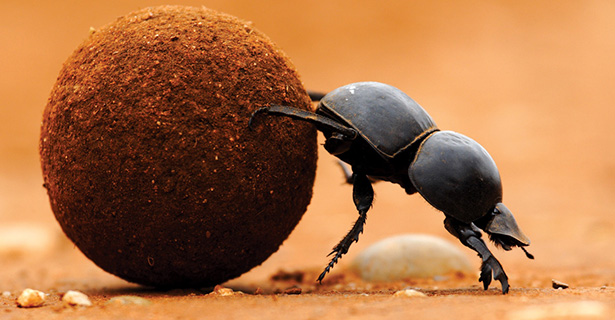
\includegraphics[height=\paperheight]{../../images/rolabosta.jpg}};
    }
\begin{frame}[b]
    \begin{center}
        \color{white}\Huge\textbf {Best description evar!}
    \end{center}
\end{frame}
}

\begin{frame}
    \begin{center}
        A única alternativa real é...
        \vfill
        \Huge \LaTeX
    \end{center}
\end{frame}

\begin{frame}
    \begin{tikzpicture}[remember picture,overlay]  
        % Posiciona o overlay na página
        \node [xshift=\paperwidth / 2,yshift=\paperheight / 2 + 3cm] at (current page.south west)
        % Adiciona a imagem, definindo seu tamanho
        {
\includegraphics[width=\paperwidth]{../../images/scream.jpg}};
    \end{tikzpicture}
\end{frame}

\begin{frame}[b]
    \frametitle{Lyx to the rescue...}
    \begin{tikzpicture}[remember picture,overlay]  
        % Posiciona o overlay na página
        \node [xshift=\paperwidth / 2,yshift=3.5cm] at (current page.south west)
        % Adiciona a imagem, definindo seu tamanho
        {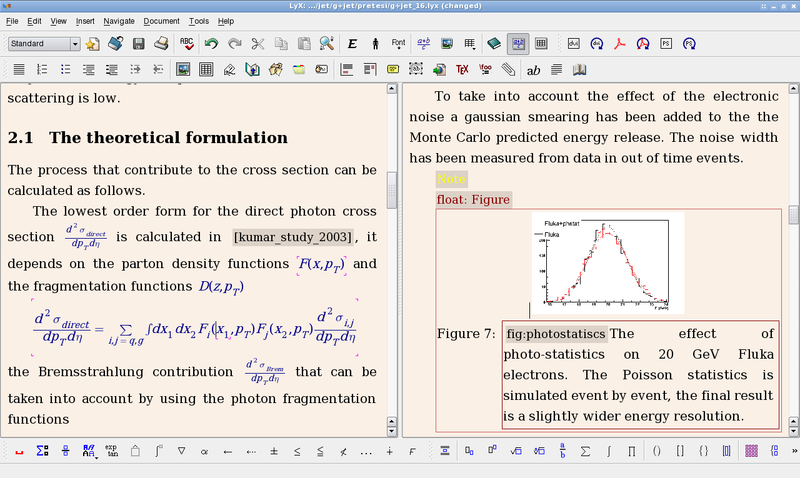
\includegraphics[width=12cm]{../../images/lyx.png}};
    \end{tikzpicture}
\end{frame}

\begin{frame}
    \frametitle{Lyx to the rescue...}
    Ou ainda...
    \begin{itemize}
        \item vi, vim, emacs (não...)
        \item Atom, Visual Studio Code
        \item ShareLaTeX, Overleaf
    \end{itemize}
\end{frame}

\begin{frame}
        \vspace{2cm}
        E como os dados são apenas texto, utilizando o \textbf{git}, e repositórios
        como \textbf{Github} e \textbf{bitbucket}, temos controle de versão, histórico
        e backup na \emph{nuvem} incluídos no pacote.
\end{frame}

\begin{frame}
    \begin{center}
    \vfill
    Tem um modelo pronto!
    \vfill
    \normalsize\url{https://github.com/rafasgj/tcc-ads-cloudbased.git}
    \vfill
    \end{center}
\end{frame}

\begin{frame}
    \frametitle{E a bibliografia?}
    \begin{itemize}
        \item{BibTeX}
        \item{Biber}
    \end{itemize}

    Ambos pdem utilizar o formato BibTeX, baseado em texto, para criar uma coleção
    de referências bibliográficas que incluem livros, artigos, congressos, \emph{websites}.
\end{frame}

{%
    \usebackgroundtemplate{
        \centering
        {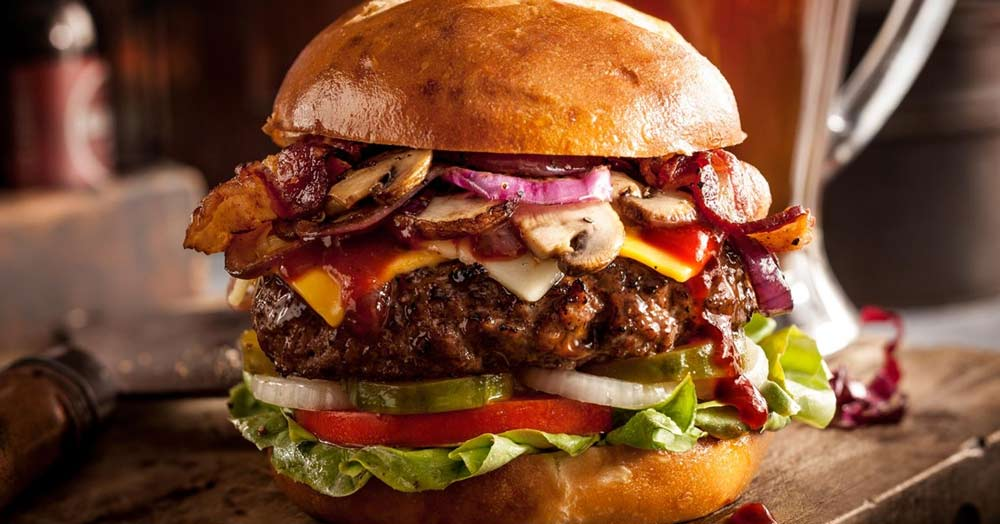
\includegraphics[height=\paperheight]{../../images/burger.jpg}};
    }
    \begin{frame}[t]
        \color{white} \huge \textbf{E a aprensentação?}
    \end{frame}
}

\begin{frame}
    \begin{center}
    \Huge Nos renderemos ao Power Point?
    \end{center}
\end{frame}

{%
    \usebackgroundtemplate{
        \centering
        \begin{tikzpicture}[remember picture,overlay]  
            % Posiciona o overlay na página
            \node [xshift=\paperwidth / 2,yshift=5cm] at (current page.south west)
            % Adiciona a imagem, definindo seu tamanho
            {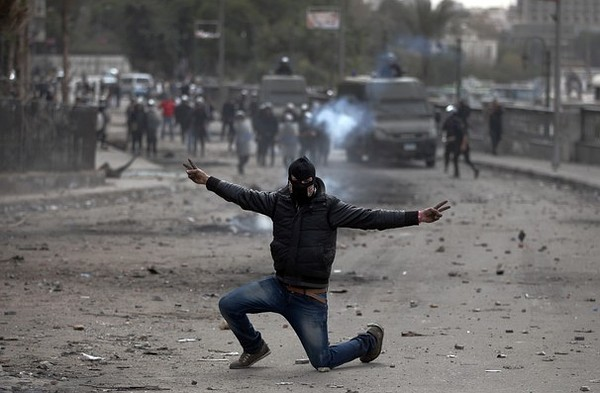
\includegraphics[width=\paperwidth]{../../images/blackblock.jpg}};
        \end{tikzpicture}
    }
\begin{frame}[t]
    \begin{center}
        \color{white} \Huge NUNCA!
    \end{center}
\end{frame}
}

\bigtitle{Então...}

{%
\usebackgroundtemplate{
    \centering
    {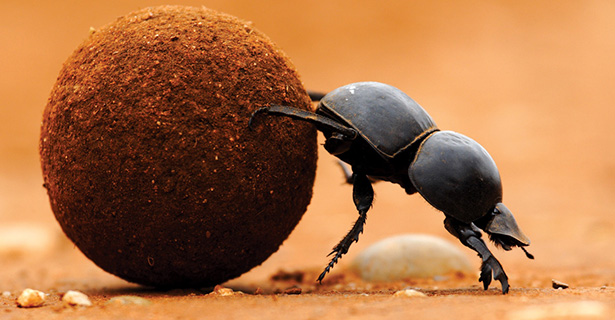
\includegraphics[height=\paperheight]{../../images/rolabosta.jpg}};
}
\begin{frame}[b]
\end{frame}
}

\bigtitle{Não pode ser...}

\begin{frame}
    \begin{center}
        \Huge \LaTeX
    \end{center}
\end{frame}

\begin{frame}[t]
    \begin{tikzpicture}[remember picture,overlay]  
        % Posiciona o overlay na página
        \node [xshift=\paperwidth / 2, yshift=\paperheight / 2] at (current page.south west)
        % Adiciona a imagem, definindo seu tamanho
        {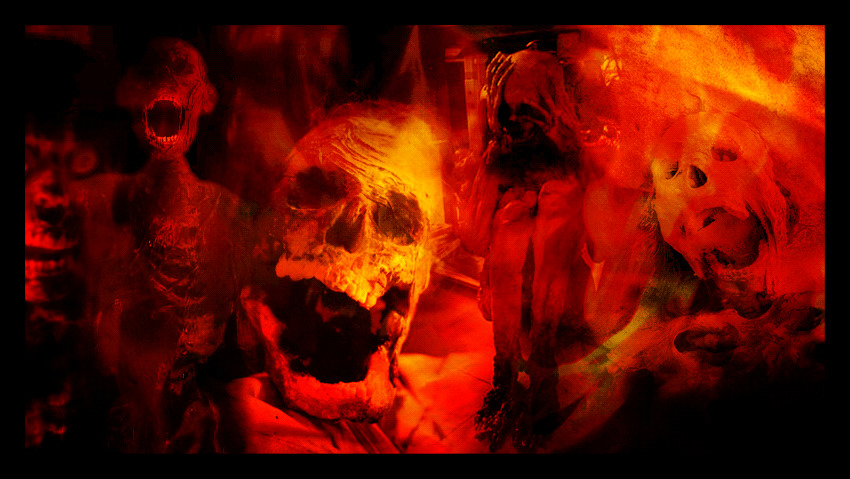
\includegraphics[height=\paperheight]{../../images/hell.jpg}};
    \end{tikzpicture}
    \vfill
    \begin{center}
    \color{white} \Huge \textbf{Não pode ser...}
    \end{center}
    \vfill
\end{frame}

\begin{frame}
    \Huge Você ainda não notou que o objetivo é não sofrer?
\end{frame}

\begin{frame}
    \frametitle{Beamer}
    Beamer é uma classe de documentos para o \LaTeX\ que facilita muito
    a criação de apresentações no estilo de \emph{slides}.
\end{frame}

\begin{frame}
    \frametitle{Tikz}

    Tikz é um pacote para o \LaTeX\ que auxilia no posicionamento de elementos
    e permite desenhar, a partir de primitivas, operações, e algoritmos iterativos.    
\end{frame}

{%
\usebackgroundtemplate{ }
\begin{frame}
    \frametitle{Exemplo do Tikz}

 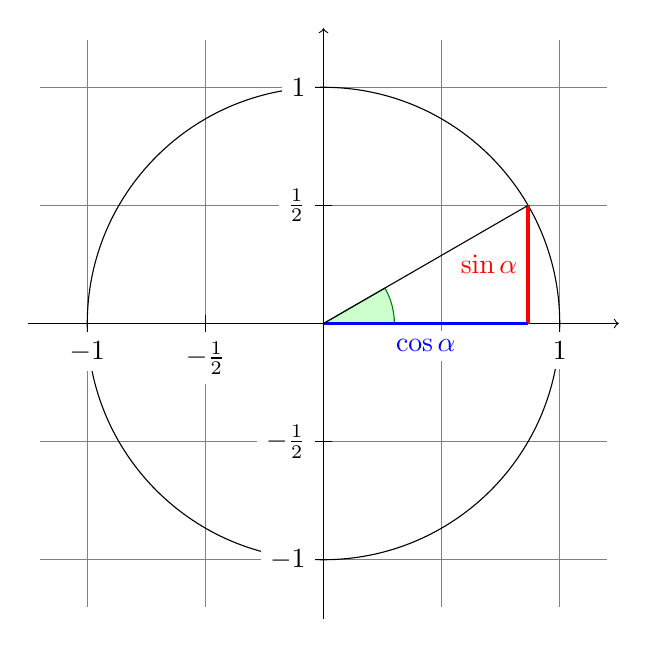
\begin{tikzpicture}[scale=3]
 \draw[step=.5cm, gray, very thin] (-1.2,-1.2) grid (1.2,1.2); 
 \filldraw[fill=green!20,draw=green!50!black] (0,0) -- (3mm,0mm) arc (0:30:3mm) -- cycle; 
 \draw[->] (-1.25,0) -- (1.25,0) coordinate (x axis);
 \draw[->] (0,-1.25) -- (0,1.25) coordinate (y axis);
 \draw (0,0) circle (1cm);
 \draw[very thick,red] (30:1cm) -- node[left,fill=white] {$\sin \alpha$} (30:1cm |- x axis);
 \draw[very thick,blue] (30:1cm |- x axis) -- node[below=2pt,fill=white] {$\cos \alpha$} (0,0);
 \draw (0,0) -- (30:1cm);
 \foreach \x/\xtext in {-1, -0.5/-\frac{1}{2}, 1} 
   \draw (\x cm,1pt) -- (\x cm,-1pt) node[anchor=north,fill=white] {$\xtext$};
 \foreach \y/\ytext in {-1, -0.5/-\frac{1}{2}, 0.5/\frac{1}{2}, 1} 
   \draw (1pt,\y cm) -- (-1pt,\y cm) node[anchor=east,fill=white] {$\ytext$};
 \end{tikzpicture}

\end{frame}
}

\begin{frame}
    \begin{center}
        Quer ver outro exemplo?
    \end{center}
\end{frame}

\finalframe[Muito Obrigado!]{\normalsize\url{mailto:rafasgj@gmail.com}}

\begin{frame}
\begin{center}
    \vfill
    Esta palestra, entre outras, tem seu código fonte disponível no repositório:
    \vfill
    https://github.com/rafasgj/tchelinux-code.git
\end{center}
\end{frame}

\end{document}

